\item Considere el generador eólico de la figura \ref{fig:eolico}. Utilizando balances integrales de momento lineal, calcule la velocidad mínima de incidencia del viento para que comience a generar potencia cuando el salto de presión es de $\Delta p$. El diámetro del círculo de los alabes  es de $D_{al}$. La eficiencia de la turbo máquina es del n. Suponga la densidad del aire de $\rho_a$.

$$\Delta p = 0,04  \text{psi} \qquad D_{al} = 27 \text{ft} \qquad n = 30 \% \qquad \rho_a = 0,076\,\text{lb/ft}^3 $$

%% Esto es una figura
\begin{figure}[h]
\centering
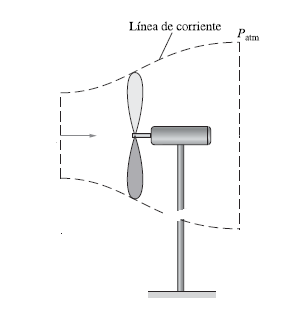
\includegraphics[width=0.4\textwidth]{g_eolico.png}
\caption{Generador eólico}
\label{fig:eolico}
\end{figure}

